\chapter{Evolução de Software}

%Possíveis tópicos (Baseados no livro: Software Maintenance – Franz Wotowa):

%Motivação
%Definição
%Classificação de Mudanças
%O Processo de Manutenção
%Leis de Lehman

Atualmente as tecnologias da informação exercem cada vez mais influência na sociedade, seja na interação entre pessoas, ou nas relações que empresas possuem com o mercado. Empresas, que possuem parte dos seus lucros associados diretamente, ou não, há sistemas de software, precisam evolui-los, seja para adequa-los à mudanças no ambiente onde estão inseridos, ou para mante-los competitivos frente aos concorrentes. Além desses fatores, quando os sistemas em questão são desenvolvidos como softwares livres, eles também precisam evoluir para que se mantenham sempre atrativos, motivando a comunidade estabelecida ao seu redor. Sistemas estagnados desmotivam usuários ou colaboradores, o que significa risco de perda de mercado ou enfraquecimento de um projeto de software livre, já que esses são feitos de colaboradores
%[modificar esse parágrafo com base no artigo challanges_sw_evolution]

Por outro lado, a manutenção desses sistemas é difícil, consome bastante tempo e recursos. Tarefas como adicionar novas funcionalidades, suporte a novos dispositivos de hardware, correção de defeitos, entre outros, se tornam mais difíceis conforme o sistema cresce e envelhece \cite{godfrey2000evolution}.

Acima foram mencionados os termos manutenção e evolução de software. Na maioria das vezes esses palavras aparecem juntas na literatura, e embora se refiram ao mesmo fenômeno, possuem ênfases diferentes. Manutenção é o ato de manter uma entidade num estado de reparo, capacidade ou disponibilidade, prevenindo-a contra falhas, mantendo a satisfação dos envolvidos ao longo do ciclo de vida do software. Já a evolução refere-se a um processo de mudança contínuo de um estado mais baixo, simples ou pior para um estado mais alto, mais complexo e melhor, refletindo a soma de todas as alterações implementadas no sistema.

%evolução de software sempre existiu, porem nao era estudada
A evolução de software foi identificada pela primeira vez no final dos anos 60, embora não denominada evolução até 1969, quando Meir M. Lehman realizou um estudo com a IBM, com a ideia de melhorar sua efetividade de programação. Apesar de não ter recebido tanta atenção e pouco impactado nas práticas de desenvolvimento dessa companhia , esse estudo fez surgir um novo campo de pesquisa, a evolução de software.
%\cite{Artigo IBM}.

Durante esses estudos, Lehman formulou as três primeiras, de um total de oito leis, conhecidas atualmente como leis de Lehman. O restante foi formulado em estudos posteriores, conforme a relevancia desse campo aumentava. O conjunto dessas oito leis estão listadas abaixo:
\begin{table}[H]
\begin{center}
    \begin{tabular}{ | l | p{4cm} | p{9cm} |}
    \hline
    Índice (Ano) & Nome & Descrição \\ \hline
    1 (1974) & Mudança contínua & Um software deve ser continuamente adaptado, caso contrário se torna progressivamente menos satisfatório. \\ \hline
    2 (1974) & Complexidade Crescente & À medida que um software é alterado, sua complexidade cresce, a menos que um trabalho seja feito para mantê-la ou diminuí-la. \\ \hline
    3 (1974) & Auto-regulação & O processo de evolução de software é auto-regulado próximo à distribuição normal com relação às medidas dos atributos de produtos e processos. \\ \hline
    4 (1978) & Conservação da estabilidade organizacional & A não ser que mecanismos de retro-alimentação tenham sido ajustados de maneira apropriada, a taxa media de atividade global efetiva num software em evolução tende a ser manter constante durante o tempo de vida do produto. \\ \hline
    5 (1991) & Conservação da Familiaridade & De maneira geral, a taxa de crescimento incremental e taxa crescimento a longo prazo tende a declinar. \\ \hline
    6 (1991) & Crescimento contínuo & O conteúdo funcional de um software deve ser continuamente aumentado durante seu tempo de vida para para manter a satisfação do usuário. \\ \hline
    7 (1996) & Qualidade decrescente & A qualidade do software será entendida como declinante a menos que o software seja rigorosamente adaptado às mudanças no ambiente operacional. \\ \hline
    8 (1971/96) & Sistema de Retro-alimentação & Processos de evolução de software são sistemas de retro-alimentação em múltiplos níves, em múltiplos laços (loops) e envolvendo múltiplos agentes. \\ \hline
    \end{tabular}
    \caption{Leis de Lehman, extraído de \cite{fernandez2008empirical}}
    \label{tab-leis-lehman}
\end{center}
\end{table}

Ao contrário das engenharias tradicionais, a engenharia de software tem em mãos um produto abstrato e intangível, o que resulta em alguns desafios inerentes aos processo de desenvolvimento. A evolução de software busca amenizar ou solucionar alguns desses desafios \cite{mens2005challenges}, entre eles:

\begin{itemize}
\item Manter e melhorar a qualidade do software;
\item Suportar evolução do modelo de desenvolvimento (não só código-fonte);
\item Manter consistência entre artefatos relacionados;
\item Integrar mudanças dentro do ciclo de desenvolvimento de software;
\item Necessidades de bons sistemas de controle de versão;
\item Integração e análise de dados de várias fontes (relatórios de erros, métricas, solicitações de mudança);
\end{itemize}

%importancia
Quando inserida ou considerada nos processos de desenvolvimento ela resulta numa excelente alternativa para evitar os sintomas do envelhecimento e inconsistencias entre o próprio software e o ambinte onde está inserido \cite{mens2005challenges}.

\section{Evolução de Software Livre}

%grande crescimento dos softwares livres em geral, a exemplo do linux
Não restam dúvidas que o desenvolvimento de softwares livres tem produzido softwares de alta qualidade com grande número de funcionalidades. Um exemplo disso é o sistema operacional Linux, que ultimamente tem experimentado um grande sucesso comercial.

Em geral sistemas desenvolvidos por meio de projetos de software livre tendem a crescer com o passar do tempo, após sucessivas releases. Esse comportamento sugere consistência com a sexta lei de Lehman, que se refere ao crescimento contínuo. Nesse sentido, além de um comportamento necessário para manter a satisfação do usuário, o crescimento contínuo de um software livre é importante para manter a motivação da comunidade estabelecida ao seu redor.

Para avaliar esse comportamento de contínuo crescimento em softwares livres Godfray \cite{godfrey2000evolution} e Mockus \cite{mockus2000case}, realizaram pesquisas, do tipo estudo de caso, baseados no sistema operacinal Linux e no servidor de aplicação Apache, respectivamente.

A \ref{Figura1} mostra o crescimento do operacional Linux desde sua primeira release, no ano de 1994. Desde então, ele é mantido por centenas de desenvolvedores que o desenvolvem em dois ramos paralelos: stable releases contendo as principais atualizações e correções de defeitos, e development releases com funcionalidades experimentais e porções de código não testado.

\graphicspath{{figuras/}}
\begin{figure}[H]
\centering
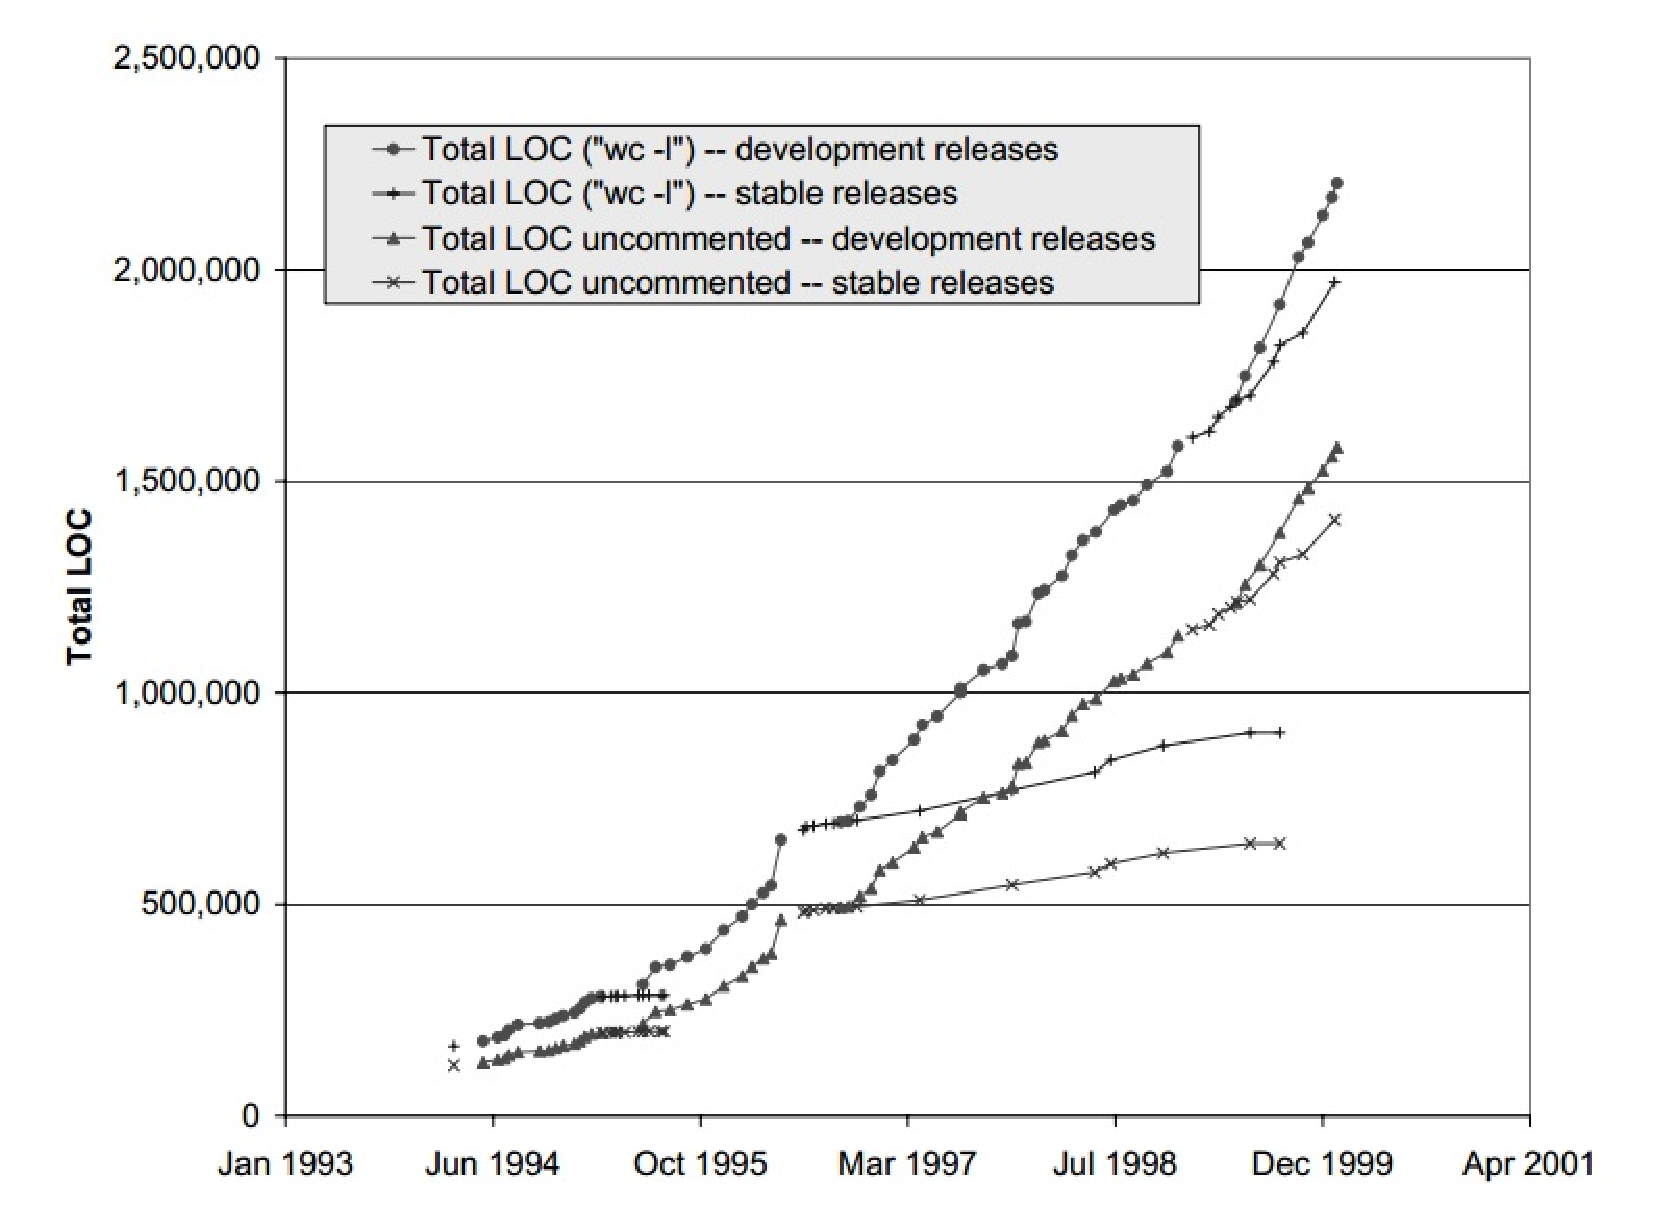
\includegraphics[width=0.6\textwidth]{linux-evolution}
\caption{Evolução do sistema operacional Linux, extraído de \cite{godfrey2000evolution}}
\label{Figura1}
\end{figure}

Os dados presentes no gráfico, até o início dos anos 2000, vão de encontro à quinta lei de Lehman, citada na \ref{tab-leis-lehman}. No gráfico, o número de linhas de código (LOC) do kernel do sistema, possui taxa de crescimento positiva, enquanto a lei afirma que ao longo do tempo a taxa de crescimento tende a diminuir.%Lehman e Turski tinham a hipótese da taxa do quadrado inverso do crescimento ao longo do tempo.











